\question[6]管道高频焊机可以对由钢板卷成的圆管的接缝实施焊接。焊机的原理如图所示,圆管通过一个接有高频交流电源的线圈,线圈所产生的交变磁场使圆管中产生交变电流,电流产生的热量使接缝处的材料熔化将其焊接。焊接过程中所利用的电磁学规律的发现者为\key{D}
\begin{center}
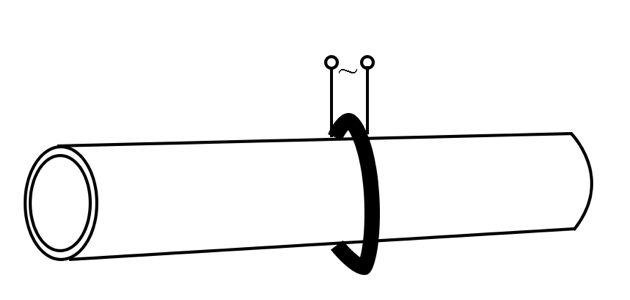
\includegraphics[]{img/image1.png}
\end{center}

\fourchoices{库仑}{霍尔}{洛伦兹}{法拉第}
\begin{solution}{4cm}

\end{solution}



\question[6]若一均匀球形星体的密度为ρ,引力常量为G,则在该星体表面附近沿圆轨道绕其运动的卫星的周期是\key{A}
\fourchoices{$\sqrt{\frac{3\pi }{G\rho}}$}{$\sqrt{\frac{4\pi }{G\rho}}$}{$\sqrt{\frac{1}{3\pi G\rho}}$}{$\sqrt{\frac{1}{4\pi G\rho}}$}
\begin{solution}{4cm}

\end{solution}



\question[6]如图,在摩托车越野赛途中的水平路段前方有一个坑,该坑沿摩托车前进方向的水平宽度为$3h,$其左边缘a点比右边缘b点高$0.5h$。若摩托车经过a点时的动能为$E_1,$它会落到坑内c点。c与a的水平距离和高度差均为h;若经过a点时的动能为$E_2,$该摩托车恰能越过坑到达b点。$\frac{E_{2}}{E_{1}}$等于\key{B}
\begin{center}
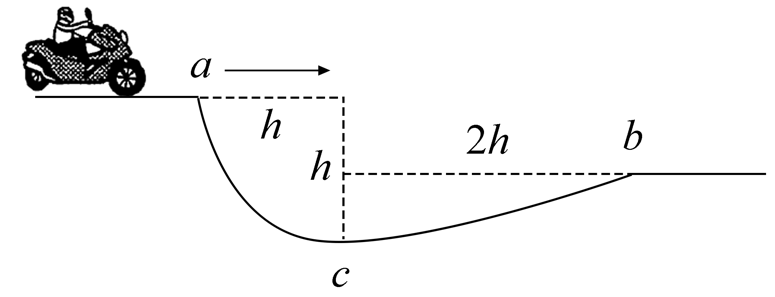
\includegraphics[]{img/image2.png}
\end{center}

\fourchoices{20}{18}{$9.0$}{$3.0$}
\begin{solution}{4cm}

\end{solution}



\question[6]CT扫描是计算机X射线断层扫描技术的简称$,CT$扫描机可用于对多种病情的探测。图(a)是某种CT机主要部分的剖面图,其中X射线产生部分的示意图如图(b)所示。图(b)中M、N之间有一电子束的加速电场,虚线框内有匀强偏转磁场;经调节后电子束从静止开始沿带箭头的实线所示的方向前进,打到靶上,产生X射线(如图中带箭头的虚线所示);将电子束打到靶上的点记为P点。则\key{D}
\begin{center}
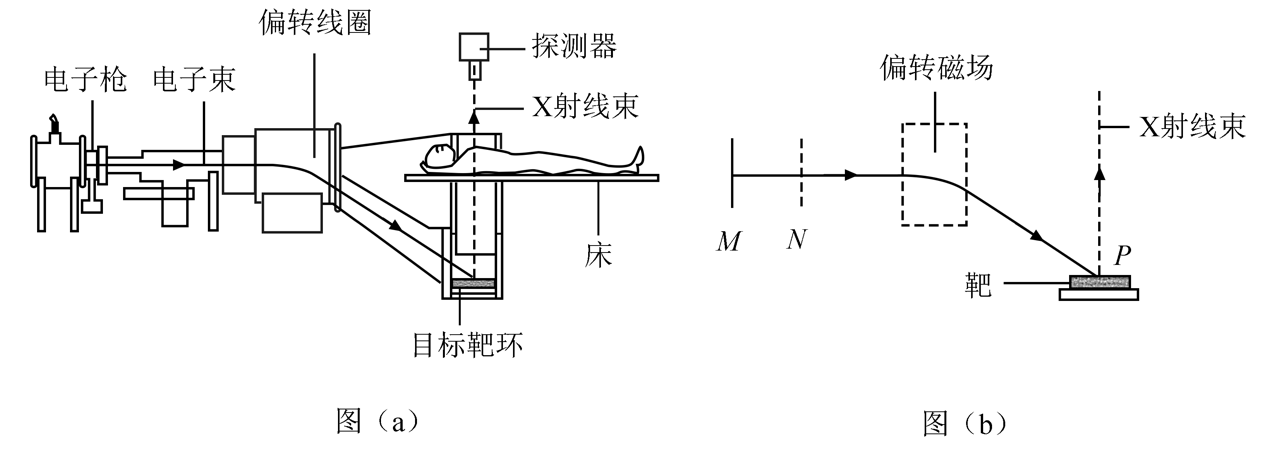
\includegraphics[]{img/image3.png}
\end{center}

\fourchoices{M处的电势高于N处的电势}{增大M、N之间的加速电压可使P点左移}{偏转磁场的方向垂直于纸面向外}{增大偏转磁场磁感应强度的大小可使P点左移}
\begin{solution}{4cm}

\end{solution}



\question[6]氘核$_1^2H$可通过一系列聚变反应释放能量,其总效果可用反应式$6_1^2H→2_2^4He+2_1^1H+2_0^1n+43.15MeV$表示。海水中富含氘,已知$1kg$海水中含有的氘核约为$1.0×10^{22}$个,若全都发生聚变反应,其释放的能量与质量为M的标准煤燃烧时释放的热量相等;已知$1kg$标准煤燃烧释放的热量约为$2.9×10^7J,1MeV=1.6×10^{-13}J,$则M约为\key{C}
\fourchoices{$40kg$}{$100kg$}{$400kg$}{$1000kg$}
\begin{solution}{4cm}

\end{solution}



\question[6]特高压输电可使输送中的电能损耗和电压损失大幅降低.我国已成功掌握并实际应用了特高压输电技术。假设从A处采用$550kV$的超高压向B处输电,输电线上损耗的电功率为$ΔP,$到达B处时电压下降了ΔU。在保持A处输送的电功率和输电线电阻都不变的条件下,改用$1100kV$特高压输电,输电线上损耗的电功率变为$ΔP^\prime,$到达B处时电压下降了$ΔU^\prime$。不考虑其他因素的影响,则\key{AD}
\fourchoices{$\Delta P^{\prime}=\frac{1}{4}\Delta P$}{$\Delta P^{\prime}=\frac{1}{2}\Delta P$}{$\Delta U^{\prime}=\frac{1}{4}\Delta U$}{$\Delta U^{\prime}=\frac{1}{2}\Delta U$}
\begin{solution}{4cm}

\end{solution}



\question[6]如图,竖直面内一绝缘细圆环的上、下半圆分别均匀分布着等量异种电荷。a、b为圆环水平直径上的两个点,c、d为竖直直径上的两个点,它们与圆心的距离均相等。则\key{ABC}
\begin{center}
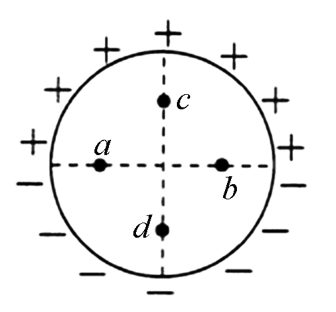
\includegraphics[]{img/image4.png}
\end{center}

\fourchoices{a、b两点的场强相等}{a、b两点的电势相等}{c、d两点的场强相等}{c、d两点的电势相等}
\begin{solution}{4cm}

\end{solution}



\question[6]水平冰面上有一固定的竖直挡板,一滑冰运动员面对挡板静止在冰面上,他把一质量为$4.0kg$的静止物块以大小为$5.0m/s$的速度沿与挡板垂直的方向推向挡板,运动员获得退行速度;物块与挡板弹性碰撞,速度反向,追上运动员时,运动员又把物块推向挡板,使其再一次以大小为$5.0m/s$的速度与挡板弹性碰撞。总共经过8次这样推物块后,运动员退行速度的大小大于$5.0m/s,$反弹的物块不能再追上运动员。不计冰面的摩擦力,该运动员的质量可能为\key{BC}
\fourchoices{$48kg$}{$53kg$}{$58kg$}{$63kg$}
\begin{solution}{4cm}

\end{solution}



